\documentclass{article}

\usepackage{lipsum}
\usepackage{project_440_550}
% Please submit it as is here, with line numbers.
% If you'd like a "less draft"-looking version for your website or something after:
%     \usepackage[final]{project_440_550}   % keeps the footer but kills line numbers,
%     \usepackage[preprint]{project_440_550}   % removes both
\usepackage{amsmath}
\usepackage{graphicx}
\providecommand{\IfPDFManagementActiveF}[1]{#1}
\usepackage[utf8]{inputenc} % allow utf-8 input
\usepackage[T1]{fontenc}    % use 8-bit T1 fonts

\usepackage[USenglish]{babel}  % there's a "canadian" option, but it's an alias for USenglish,
                               % and for some reason it makes csqoutes behave differently...
\usepackage{csquotes}       % smarter handling of quotes (used by biblatex)

\usepackage{booktabs}       % professional-quality tables
\usepackage{amsfonts}       % blackboard math symbols
\usepackage{nicefrac}       % compact symbols for 1/2, etc.
\usepackage{microtype}      % microtypography
\usepackage{xcolor}         % colors
\usepackage{hyperref}       % hyperlinks
\usepackage{url}            % simple URL typesetting

% I recommend the biblatex package.
% If you hate it for some reason, though, you can use natbib instead:
% comment out this block and uncomment the next one.

\usepackage[style=authoryear,maxbibnames=30,natbib]{biblatex}
\addbibresource{refs.bib}
\renewbibmacro{in:}{}  % drops a silly "In:" from biblatex format
\DeclareDelimFormat{nameyeardelim}{\addspace} % remove a comma i dislike, doesn't matter
\DeclareNameAlias{sortname}{given-family}  % avoid kinda-weird bib printing order

%\usepackage[round]{natbib}
%\newcommand{\printbibliography}{\bibliographystyle{plainnat}\bibliography{refs}}

\usepackage{tikz}
\usetikzlibrary{shapes.geometric, positioning, fit, backgrounds, arrows.meta, decorations.pathreplacing, calc}
\usepackage[capitalize,noabbrev]{cleveref}

\newcommand{\R}{\mathbb{R}}
\newcommand{\N}{\mathbb{N}}
\newcommand{\E}{\mathbb{E}}
\newcommand{\K}{\mathcal{K}}
\newcommand{\prox}{\operatorname{prox}}

% Theorem environments
\newtheorem{theorem}{Theorem}[section]
\newtheorem{definition}{Definition}[section]
\newtheorem{lemma}{Lemma}[section]
\newtheorem{assumption}{Assumption}


\title{Benchmark and Survey on Vision Unlearning}


% The \author macro works with any number of authors. There are two commands
% used to separate the names and addresses of multiple authors: \And and \AND.
%
% Using \And between authors leaves it to LaTeX to determine where to break the
% lines. Using \AND forces a line break at that point. So, if LaTeX puts 3 of 4
% authors names on the first line, and the last on the second line, try using
% \AND instead of \And before the third author name.

\author{%
  Inzaghi Moniaga\\
  \texttt{inzaghi@student.ubc.ca}
  \And
  Kevin K Thomas\\
  \texttt{kevinktv@cs.ubc.ca}
}

\begin{document}
\maketitle
\begin{abstract}
We present a survey and empirical benchmark of approximate machine unlearning algorithms against a retraining baseline. We evaluate these methods on two image classification datasets, CIFAR-10 and MUFAC, using an evaluation protocol inspired by the NeurIPS 2023 Machine Unlearning Competition [\cite{neurips-2023-machine-unlearning}].

Specifically, we consider four algorithms: SCRUB, DELETE, the 2023 Kaggle first-place solution (Fanchuan), and the 2023 Kaggle second-place solution (MSG). Our study provides a comparative analysis of their performance in terms of forgetting quality, utility retention, and computational efficiency.
\end{abstract}

\section{Introduction}
As machine learning models are increasingly deployed in real-world systems, the ability to unlearn specific data from trained models has become a critical requirement for privacy and security reasons. Machine unlearning refers to the process of removing the influence of specific data points from a trained model, effectively forgetting that data. 
In 2023, California signed the DELETE Act [\cite{delete_act}], which requires data brokers to delete personal information upon request. Bill C-27, which is currently being debated in the Canadian parliament, plans to modernize privacy laws, especially in the context of AI and machine learning. These laws highlight the importance of machine unlearning and the need for efficient algorithms to achieve it.

Ideally, unlearning requires retraining a model from scratch on the remaining data to ensure complete removal. However, because full retraining is computationally prohibitive for large datasets, efficient approximate algorithms are increasingly necessary.

We benchmark four recent approximate unlearning algorithms on image classification tasks:
SCalable Remembering and Unlearning unBound (SCRUB) [\cite{kurmanji2023unboundedmachineunlearning}], DEcoupLEd Distillation To Erase (DELETE) [\cite{zhou2025decoupleddistillationerasegeneral}], the 2023 Kaggle 1st place winner (Fanchuan) [\cite{2023-winner}], and the 2023 Kaggle 2nd place winner (MSG) [\cite{2023-second-place}] where the acronym MSG (Masked Small Gradients) follows the naming convention used in \citet{cadet2025}. 
We evaluate these methods on two image classification datasets: CIFAR-10 [\cite{Krizhevsky09learningmultiple}] and MUFAC [\cite{choi2023machine}]. We use an evaluation metric inspired by the NeurIPS 2023 Machine Unlearning Competition, which combines measures of forgetting quality, utility retention, and runtime efficiency into a single score.

\section{Related Work}
\textbf{Machine Unlearning.} In machine unlearning, our goal is to remove the influence of specific data points from a trained model \citep{bourtoule2021machine, zhang2023review}. \citet{cao2015towards} proposed a method of unlearning based on reformulating the learning algorithm into a summation-based form and unlearning by subtracting contributions of specific summands. However, this approach requires that the learning algorithm be expressible in a summation form which is not feasible for most modern deep learning models. 
\cite{bourtoule2021machine} proposed a method called SISA (Sharded, Isolated, Sliced, and Aggregated) training, which partitions the training data into shards and trains separate models on each shard. To unlearn a data point, only the model trained on the shard containing that data point needs to be retrained. However, as the number of shards increases, the performance of the model degrades. Recently, several new algorithms have been proposed that aim to achieve better performance while still being efficient and scalable \citep{cadet2025, kurmanji2023unboundedmachineunlearning, zhou2025decoupleddistillationerasegeneral}.

\textbf{Evaluation Metrics.} Ideally, evaluating unlearning algorithms requires measuring how close the distribution of the unlearned model is to the distribution of a model retrained from scratch on the remaining data. However, this is not feasible in practice since we do not have access to the true, distributions. Evaluation metrics are usually based on the following components \citep{li2025overview}: 

\begin{itemize}
    \item \textbf{Utility.} This measures how well the model performs on data that should be retained. It is typically evaluated using standard metrics such as accuracy on the retained set and a held-out test set.
    
    \item \textbf{Forgetting quality (indistinguishability).} This evaluates whether the influence of the removed samples has been eliminated. The model produced by the unlearning algorithm must be indistinguishable from a model retrained from scratch on the remaining data. 
    
    \item \textbf{Efficiency.} This captures the computational advantage of the unlearning algorithm compared to full retraining. 
    
    \item \textbf{Privacy leakage.} This assesses whether information about the removed data can still be extracted from the model. 
\end{itemize}
In this project, we focus on the first three components and use the evaluation protocol from the NeurIPS 2023 Machine Unlearning Competition \citep{neurips-2023-machine-unlearning}.

\section{Problem Setup} \label{sec:problem_setup}
We base our problem setup on \cite{li2025overview}. We begin with some notation and definitions. Let $Z$ be the set of all data points and $Z^*$ be the set of all possible training datasets. Let $H$ be the set of all possible hypotheses (i.e. parameters). We define
\begin{definition}[Learning Algorithm]
    A learning algorithm $A: Z^* \to H$ maps a training dataset to a hypothesis. If $D \in Z^*$, then $A(D)$ is the model obtained by training on $D$.
\end{definition}
\begin{definition}[Unlearning Algorithm]
    An unlearning algorithm $U: H \times Z^* \times Z^* \to H$ takes a trained model, the original training dataset, and a subset of data points to unlearn, and produces a new model. Specifically, if $h = A(D)$ is the model trained on $D$, and $S \subseteq D$ is the subset of data points to unlearn, then $U(h, D, S)$ is the model obtained by unlearning $S$ from $h$.
\end{definition}
Note that both $A$ and $U$ can be randomized algorithms that define a distribution over the hypothesis space $H$.

Suppose we have a training dataset $D \in Z^*$ and a subset of data points $S \subseteq D$ that we wish to unlearn (called the forget set). Let $D' = D \setminus S$ (called the retain set). The goal of machine unlearning is to create an unlearning algorithm $U$ such that the distribution of $U(A(D), D, S)$ is close to the distribution of $A(D')$ (i.e. retraining the original model on the smaller retain set).
i.e.
\begin{equation}
    \Pr[A(D')] \approx \Pr[U(A(D), D, S)]
\end{equation} 
Of course, we do not have access to the true distributions so there are several metrics that have been proposed to evaluate the performance of unlearning algorithms. In this project, we use the evaluation protocol from the NeurIPS 2023 Machine Unlearning Competition. Additional details about the evaluation protocol are described in \Cref{subsec:evaluation}.

\section{Unlearning Algorithms and Evaluation Metric}
Below, we briefly summarize the unlearning algorithms that we benchmarked in this project.

\subsection{SCRUB}
\textbf{SCalable Remembering and Unlearning unBound (SCRUB)} [\cite{kurmanji2023unboundedmachineunlearning}]: SCRUB utilizes a teacher-student framework where both models are initialized with identical weights. The goal is for the student to "obey" the teacher for the retain set and "disobey" the teacher for the forget set. 
To achieve this, SCRUB uses a loss function that encourages the student to produce similar outputs to the teacher on the retain set, while producing different outputs on the forget set. The final component of the loss function is the loss purely on the retain set, which encourages the student to perform well on it. By optimizing this loss function, SCRUB effectively unlearns the forget set while retaining performance on the retain set.

\subsection{DELETE}
\textbf{DEcoupLEd Distillation To Erase (DELETE)} [\cite{zhou2025decoupleddistillationerasegeneral}]: DELETE is also an unlearning algorithm that is based on the knowledge distillation/teacher-student framework. In the paper, they showed that the KL between the target probability distribution (i.e. full retrain) and the unlearned model can be broken into two parts: the KL on the forget set and the KL on the retain set. The original pretrained model is used as the teacher, and the output distribution is modified by masking out the specific class to be forgotten. Then the student model tries to learn this modified masked distribution. 
This ensures that the student model forgets the specific class while still retaining performance on the other classes. 

 
\subsection{Kaggle 2023 Winner}
\textbf{Kaggle 2023 Winner (Fanchuan)} [\cite{2023-winner}]: Fanchuan operates in two stages: first, it minimizes the KL divergence of the model's output on the forget set and a uniform distribution. This encourages the model to produce less confident predictions on the forget set. In the second stage, the algorithm performs adversarial fine-tuning using contrastive learning to push the forget samples away from the retain samples in the feature space. They simultaneously also reduce the cross-entropy loss on the retain set to preserve performance on the retain set. 

\subsection{Kaggle 2023 runner up (Masked-Small-Gradients)}
\textbf{Masked-Small-Gradients (MSG)} [\cite{2023-second-place}]: In MSG, the unlearning process hinges on identifying weights in the model that influence both the forget set and the retain set and do not distinguish between them. The algorithm first computes the gradients of the loss with respect to the model parameters for both the forget set and the retain set. Weights with small gradient magnitudes indicate that the specific weight. 
does not help distinguish between the forget and retain sets. Hence, MSG reinitializes these weights and then retrains these weights on the retain set while keeping the other weights fixed. This approach avoids a full retraining by only updating a subset of the model parameters that are deemed less important for distinguishing the forget set from the retain set.

\section{Experimental Setup}
\begin{figure}[htbp]
    \centering
    \resizebox{\textwidth}{!}{%
    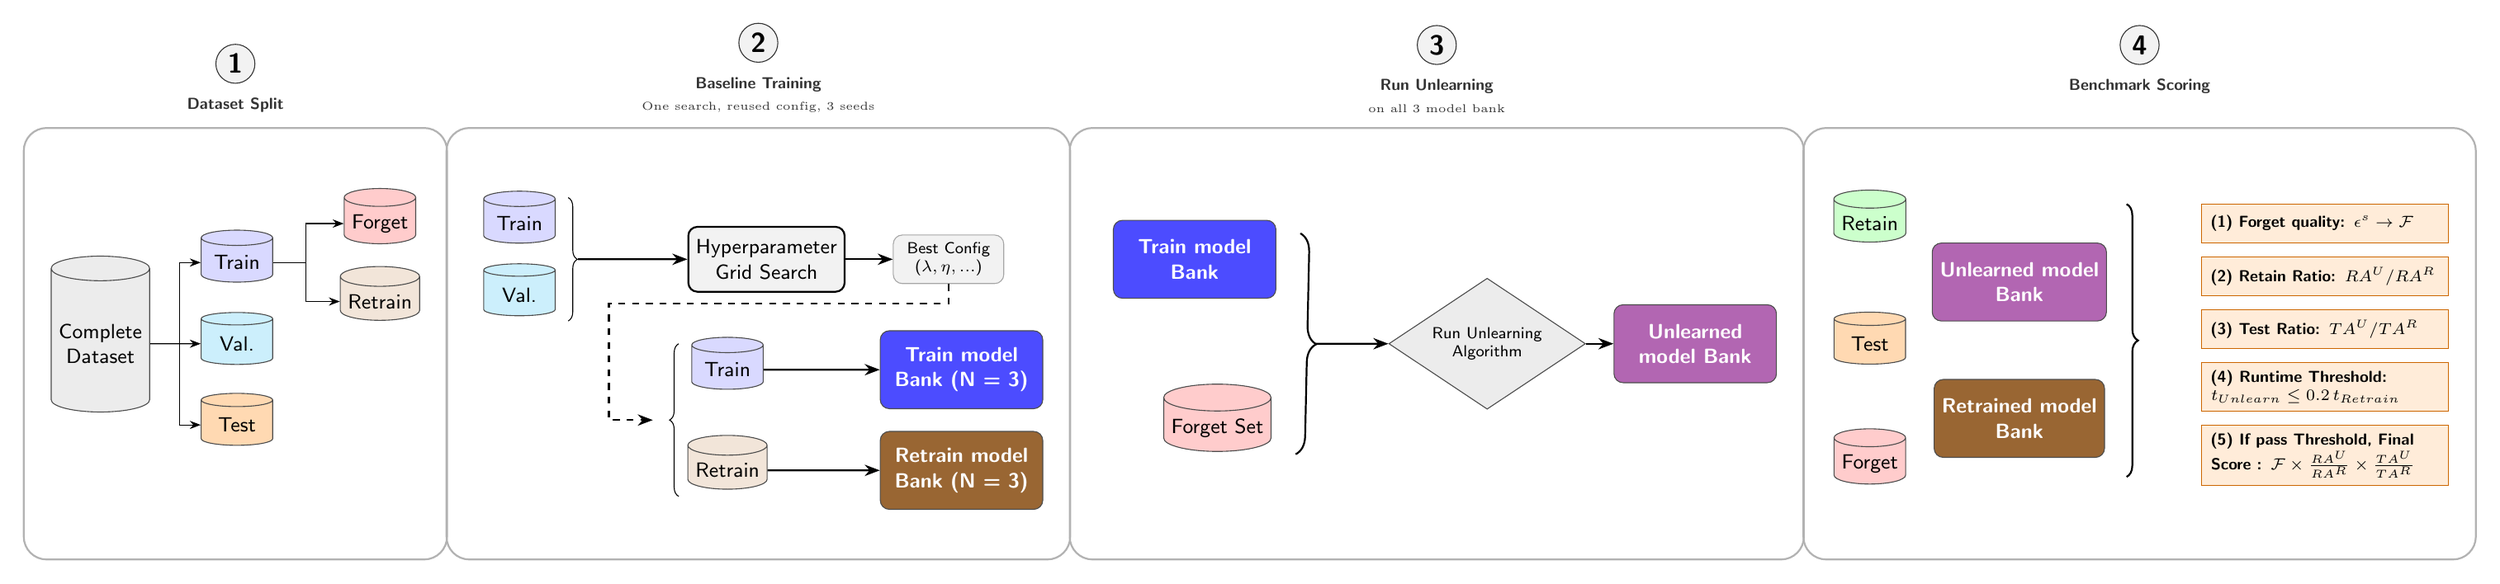
\begin{tikzpicture}[
        >=Stealth,
        font=\sffamily\small,
        db/.style={cylinder, shape border rotate=90, aspect=0.25, draw=black!70, minimum height=0.8cm, minimum width=1.1cm, align=center},
        model/.style={rectangle, rounded corners, draw=black!70, minimum height=1.2cm, minimum width=1.8cm, align=center, text=white, font=\sffamily\bfseries\small},
        action/.style={diamond, aspect=1.5, draw=black!70, minimum width=1.5cm, align=center, font=\sffamily\scriptsize},
        note/.style={rectangle, rounded corners, draw=gray!70, fill=gray!10, minimum height=0.7cm, minimum width=1.7cm, align=center, font=\sffamily\scriptsize},
        % --- UPDATED METRIC STYLE FOR HIGHER VISIBILITY ---
        metric/.style={rectangle, draw=orange!80!black, fill=orange!15, text=black, minimum height=0.6cm, minimum width=3.8cm, align=center, font=\sffamily\scriptsize\bfseries},
        % --------------------------------------------------
        box/.style={rectangle, draw=gray!60, thick, rounded corners=10pt, minimum height=6.2cm, inner sep=12pt},
        hdr/.style={rectangle, align=center, fill=white, font=\sffamily\scriptsize\bfseries, text=black!80},
        circ/.style={circle, draw=black!80, font=\sffamily\large\bfseries, inner sep=2pt, minimum size=0.6cm, fill=gray!10},
        colTrain/.style={fill=blue!15, text=black},
        colRetain/.style={fill=green!20, text=black},
        colForget/.style={fill=red!20, text=black},
        colRetrainData/.style={fill=brown!20, text=black},
        colVal/.style={fill=cyan!20, text=black},
        colTest/.style={fill=orange!30, text=black},
        colOrig/.style={fill=blue!70, text=white},
        colRetrain/.style={fill=brown!80!black, text=white},
        colUnlearn/.style={fill=violet!60, text=white}
    ]

        \begin{scope}[local bounding box=phase1_inner]
            \path (0, 2.9) -- (0, -2.9);

            \node[db, fill=gray!15, minimum height=2.4cm, minimum width=1.5cm] (task_main) at (0,0) {Complete\\Dataset};

            \coordinate (d_top) at ($(task_main.center) + (0.9, 1.2)$);
            \coordinate (d_bot) at ($(task_main.center) + (0.9, -1.2)$);

            \node[db, colTrain]       (db_train1)   at (2.1,  1.25) {Train};
            \node[db, colVal]         (db_val1)     at (2.1,  0.00) {Val.};
            \node[db, colTest]        (db_test1)    at (2.1, -1.25) {Test};
            \node[db, colForget]      (db_forget1)  at (4.3,  1.85) {Forget};
            \node[db, colRetrainData] (db_retrain1) at (4.3,  0.65) {Retrain};

            \draw[->] (task_main.east) -- ++(0.45,0) |- (db_train1.west);
            \draw[->] (task_main.east) -- ++(0.45,0) -- (db_val1.west);
            \draw[->] (task_main.east) -- ++(0.45,0) |- (db_test1.west);
            \draw[->] (db_train1.east) -- ++(0.50,0) |- (db_forget1.west);
            \draw[->] (db_train1.east) -- ++(0.50,0) |- (db_retrain1.west);


        \end{scope}

        \node[box, fit=(phase1_inner)] (box1) {};
        \node[hdr, above=0.1cm of box1] (hdr1) {Dataset Split};
        \node[circ, above=0.1cm of hdr1] {1};


\begin{scope}[shift={(box1.east)}, xshift=0.4cm, local bounding box=phase2_inner]
    \path (0, 2.9) -- (0, -2.9);

    % --- 1. Grid Search Phase ---
    \node[db, colTrain] (p2_train_search) at (0.7,  1.85) {Train};
    \node[db, colVal]   (p2_val_search)   at (0.7,  0.75) {Val.};
    \coordinate (p2_s_top) at ($(p2_train_search.center) + (0.75, 0.4)$);
    \coordinate (p2_s_bot) at ($(p2_val_search.center) + (0.75, -0.4)$);
    
    \draw[decorate,decoration={brace,amplitude=4pt}] (p2_s_top) -- (p2_s_bot)
        node[midway, right=0.15cm, align=center, font=\sffamily\bfseries] {};

    \node[draw, thick, rounded corners, fill=gray!10, align=center, minimum height=1cm] 
        (p2_search) at (4.5, 1.30) {Hyperparameter\\Grid Search};
    
    \draw[->, thick] ($(p2_s_top)!0.5!(p2_s_bot) + (0.15, 0)$) -- (p2_search.west);

    \node[note] (p2_cfg) at (7.3, 1.30) {Best Config\\($\lambda, \eta, ...$)};
    \draw[->, thick] (p2_search.east) -- (p2_cfg.west);



    % --- 2. Final Training Phase ---
    \node[db, colTrain] (p2_train_run) at (3.9, -0.40) {Train};
    \node[model, colOrig, minimum width=2.5cm] (p2_train_bank) at (7.5, -0.40) {Train model\\Bank (N = 3)};
    \draw[->, thick] (p2_train_run.east) -- (p2_train_bank.west);

    \node[db, colRetrainData] (p2_retrain_run) at (3.9, -1.95) {Retrain};
    \node[model, colRetrain, minimum width=2.5cm] (p2_retrain_bank) at (7.5, -1.95) {Retrain model\\Bank (N = 3)};
    \draw[->, thick] (p2_retrain_run.east) -- (p2_retrain_bank.west);

    \coordinate (p2_r_top) at ($(p2_train_run.center) - (0.75, -0.4)$);
    \coordinate (p2_t_bot) at ($(p2_retrain_run.center) - (0.75, +0.4)$);

    % 1. Changed order to (p2_t_bot) -- (p2_r_top) to make it a left-facing brace
    % 2. Added a coordinate 'p2_brace_mid' to the node for the arrow to target
    \draw[decorate,decoration={brace,amplitude=4pt}] (p2_t_bot) -- (p2_r_top)
        node[midway, left=0.15cm] (p2_brace_mid) {};
        
    % 3. Draw a zig-zag arrow from Best Config to the brace
    \draw[->, thick, dashed] (p2_cfg.south) 
        -- ++(0, -0.3)                                 % 1. Small drop down
        -| ($(p2_brace_mid) + (-0.8, 0)$)              % 2. Move LEFT past the brace
        |- (p2_brace_mid.west);                        % 3. Move DOWN and RIGHT into the tip
\end{scope}

        \node[box, fit=(phase2_inner)] (box2) {};
        \node[hdr, above=0.1cm of box2] (hdr2) {Baseline Training\\[0.5ex] \normalfont\tiny One search, reused config, 3 seeds};
        \node[circ, above=0.1cm of hdr2] {2};



\begin{scope}[shift={(box2.east)}, xshift=0.4cm, local bounding box=phase3_inner]
        \path (0, 2.9) -- (0, -2.9);

        % --- 1. Inputs (Aligned vertically) ---
        \node[model, colOrig, minimum width=2.5cm] (p3_base) at (1.5, 1.30) {Train model\\Bank};
        \node[db, colForget] (p3_forget) at (1.85, -1.30) {Forget Set};

        % --- 2. Positioning the Brace ---
        % We define coordinates to the right of the input nodes
        \coordinate (p3_brace_top) at ($(p3_base.east) + (0.3, 0.4)$);
        \coordinate (p3_brace_bot) at ($(p3_forget.east) + (0.3, -0.4)$);

        % Draw the right-facing brace (Top to Bottom path = Right-facing)
        \draw[decorate, decoration={brace, amplitude=8pt, raise=2pt}, thick] 
            (p3_brace_top) -- (p3_brace_bot)
            node[midway, xshift=0.6cm] (p3_brace_tip) {};

        % --- 3. Process & Output (Centered to the brace tip) ---
        % Y-coordinate 0.65 is exactly between 1.3 and 0.0
        \node[action, fill=gray!15, minimum height=1cm] (p3_run) at (6.0, 0) {Run Unlearning\\Algorithm};
        
        \node[model, colUnlearn, minimum width=2.5cm] (p3_candidate) at (9.2, 0) {Unlearned\\model Bank};

        % --- 4. Final Arrows ---
        % From brace tip to algorithm
        \coordinate (p3_top) at ($(p3_brace_tip.center) - (0.25, 0)$);
        \draw[->, thick] (p3_top) -- (p3_run.west);
        
        % From algorithm to candidate
        \draw[->, thick] (p3_run.east) -- (p3_candidate.west);

    \end{scope}

        \node[box, fit=(phase3_inner)] (box3) {};
        \node[hdr, above=0.1cm of box3] (hdr3) {Run Unlearning\\[0.5ex] \normalfont\tiny on all 3 model bank};
        \node[circ, above=0.1cm of hdr3] {3};


\begin{scope}[shift={(box3.east)}, xshift=0.4cm, local bounding box=phase4_inner]
            \path (0, 2.9) -- (0, -2.9);

            \node[db, colRetain] (p4_retain) at (0.6,  1.85) {Retain};
            \node[db, colTest]   (p4_test)   at (0.6,  0) {Test};
            \node[db, colForget] (p4_forget) at (0.6, -1.85) {Forget};

            \node[model, colUnlearn, minimum width=2.5cm] (p4_candidate) at (2.9,  0.95) {Unlearned model\\Bank};
            \node[model, colRetrain, minimum width=2.5cm] (p4_reference) at (2.9, -1.15) {Retrained model\\ Bank};

            % 1. Place the first node at a fixed coordinate
            \node[metric, text width=3.5cm, align=left] (m1) at (7.6,  1.85) {\textbf{(1)} Forget quality: $\epsilon^s \rightarrow \mathcal{F}$};
            
            % 2. Chain the rest of the nodes using 'below=0.2cm of ...' for perfectly equal gaps
            \node[metric, text width=3.5cm, align=left, below=0.2cm of m1] (m2) {\textbf{(2)} Retain Ratio: $RA^U/RA^R$};
            \node[metric, text width=3.5cm, align=left, below=0.2cm of m2] (m3) {\textbf{(3)} Test Ratio: $TA^U/TA^R$};
            \node[metric, text width=3.5cm, align=left, below=0.2cm of m3] (m4) {\textbf{(4)} Runtime Threshold: $t_{Unlearn} \leq 0.2\,t_{Retrain}$};
            \node[metric, text width=3.5cm, align=left, below=0.2cm of m4] (m5) {\textbf{(5)} If pass Threshold, Final Score : $\mathcal{F} \times \frac{RA^U}{RA^R} \times \frac{TA^U}{TA^R}$};

            \coordinate (m_left_top) at (4.55, 2.15);
            \coordinate (m_left_bot) at (4.55, -2.05);
            
            % 3. Added 'thick' (you can also use 'very thick' or 'line width=1.5pt' for even more weight)
            \draw[thick, decorate,decoration={brace,amplitude=5pt}] (m_left_top) -- (m_left_bot) coordinate[midway] (p4_metric_mid);

        \end{scope}

        \node[box, fit=(phase4_inner)] (box4) {};
        \node[hdr, above=0.1cm of box4] (hdr4) {Benchmark Scoring\\[0.5ex] \normalfont\tiny};
        \node[circ, above=0.1cm of hdr4] {4};

    \end{tikzpicture}%
    }
    \caption{Overview of the benchmark pipeline. Data is partitioned (Phase 1) to build matched Train and Retrain model banks using a shared hyperparameter configuration (Phase 2). After applying unlearning algorithms (Phase 3), the resulting models are evaluated against the retrained baselines (Phase 4). Final scores are strictly gated by a runtime efficiency threshold ($t_{Unlearn} \leq 0.2\,t_{Retrain}$).}
\label{fig:pipeline}
\end{figure}


Figure~\ref{fig:pipeline} summarizes our benchmark pipeline. For each dataset, we first construct deterministic \texttt{train}, \texttt{val}, \texttt{test}, \texttt{forget}, and \texttt{retrain} splits to prevent data leakage between tuning and evaluation. We then run a single hyperparameter grid search for ResNet-18 (no-pretrained weights), reuse the selected configuration for both the Train and Retrain model banks, and evaluate each setting over matched three-seed runs. This design keeps the comparison fair by avoiding extra tuning for either bank, reduces variance from random initialization, and provides a clean retrained reference trained only on \texttt{retrain} against which approximate unlearning methods can be judged.

Our code is implemented in PyTorch and is available at \url{https://github.com/Kevinktv/CPSC550_Project}.

\subsection{Model architecture and datasets}
For our base architecture, we utilize a ResNet-18 model with no pre-trained weights. 

We evaluate the unlearning algorithms across three primary image classification datasets: Kaggle Machine Unlearning Dataset \citep{neurips-2023-machine-unlearning}, CIFAR-10 \citep{Krizhevsky09learningmultiple}, MUFAC \citep{choi2023machine}.

For the unlearning task, the training data is divided into two mutually exclusive sets:
\begin{enumerate}
    \item \textbf{Forget Set ($S$):} A subset of the training data selected to be unlearned. Our generation pipeline builds a mixed-label unlearning task that proportionally targets specific classes or targets a globally defined forget percentage.
    \item \textbf{Retain Set ($D \setminus S$):} The remaining data from the training partition, representing the data the model must preserve.
\end{enumerate}

Held-out validation to tune hyperparameters and test sets are strictly maintained to measure generalization during unlearning. Full details of this tuning process can be found in \Cref{fig:hyperparameterTuning}.


% To accommodate smaller image resolutions without suffering from spatial detail collapse, the ResNet-18 stem is modified for $32 \times 32$ inputs by replacing the initial $7 \times 7$ convolution with a $3 \times 3$ kernel and swapping the max-pooling layer with an identity mapping. For larger inputs, the standard ResNet-18 stem is preserved.

\subsection{Evaluation}\label{subsec:evaluation}
To evaluate the performance of the unlearning methods, we utilize an evaluation criterion that follows the \textbf{NeurIPS 2023 Machine Unlearning Competition} methodology \citep{neurips-2023-machine-unlearning}.

The goal is to measure how closely an unlearned model matches a model retrained from scratch on the retained dataset $D \setminus S$. A successful unlearning method should produce outputs that are indistinguishable from this retrained baseline while preserving utility and improving efficiency.



\subsubsection*{Step 1: Estimating Per-Example Indistinguishability ($\epsilon^s$)}

As mentioned in \Cref{sec:problem_setup}, it is not possible to directly compute indistinguishability; hence, we approximate it. We first compute per-example indistinguishability, that is, whether we can distinguish between the outputs of the unlearned and retrained model on that example. For every example $s \in S$, we apply various ''attacks'' on the model outputs to see whether we can distinguish the models. This yields a False Positive Rate (FPR) and False Negative Rate (FNR). 
\begin{itemize}
    \item \textbf{False Positive Rate (FPR):} Probability of incorrectly classifying a retrained model as unlearned,
    \item \textbf{False Negative Rate (FNR):} Probability of incorrectly classifying an unlearned model as retrained.
\end{itemize}
High FPR and FNR indicate that attacks cannot reliably distinguish between the two models, implying strong indistinguishability. We convert these rates into one final score $\epsilon^s$, where a smaller $\epsilon^s$ indicates better indistinguishability. We use the strongest (worst-case) attack for each example.


\subsubsection*{Step 2: Calculating Forgetting Quality ($\mathcal{F}$)}
Once $\epsilon^s$ is calculated, we discretize it into bins, $n(s)$, where smaller $\epsilon^s$ are placed in the smaller bin numbers. We then assign scores to each bin using a scoring function $\mathcal{H}(s)$:
\begin{equation}
    \mathcal{H}(s) = \frac{2}{2^{n(s)}}
\end{equation}
This assigns higher scores to samples with smaller $\epsilon^s$ values. The total forgetting quality, $\mathcal{F}$, is defined as the average of these scores across all examples in the forget set:
\begin{equation}
    \mathcal{F} = \frac{1}{|S|} \sum_{s \in S} \mathcal{H}(s)
\end{equation}

\subsubsection*{Step 3: Calculating Model Utility}
We measure the utility of a model, $O$, as the accuracy on the retain set ($D \setminus S$) and a held-out test set ($T$). 
\begin{align}
    \text{Retain Accuracy (RA)}&: \quad RA(O) = \frac{1}{|O|} \sum_{i=1}^{|O|} Acc(O_i, D \setminus S) \\
    \text{Test Accuracy (TA)}&: \quad TA(O) = \frac{1}{|O|} \sum_{i=1}^{|O|} Acc(O_i, T)
\end{align}
We compute these average accuracies for the candidate unlearned models ($RA^U$ and $TA^U$) and compare them directly against the ideal retrained models ($RA^R$ and $TA^R$).

\subsubsection*{Step 4: The Final Combined Score}
Unlearning algorithms must first pass a hard threshold for time efficiency (strictly faster than retraining). If the candidate passes the efficiency cutoff, the mathematical components are combined into a final performance score:
\begin{equation}
    \text{Score} = \mathcal{F} \times \frac{RA^U}{RA^R} \times \frac{TA^U}{TA^R}
\end{equation}
This final formulation scales the forgetting quality $\mathcal{F}$ by the utility ratios. It explicitly penalizes the score if the unlearned model performs worse than the perfectly retrained model on the retain or test distributions. The resulting score is strictly bounded in the range $[0, 1]$:
\begin{itemize}
    \item A score approaching \textbf{1.0} indicates a flawless unlearner that mimics a retrained model without utility loss.
    \item A score approaching \textbf{0.0} signifies that the algorithm either failed to effectively forget the targeted data, completely collapsed the model's accuracy, or failed the runtime efficiency requirements.
\end{itemize}


\section{Discussion and future work}
\begin{table}[htbp]
    \centering
    \small
    \caption{Benchmark summary for CIFAR-10 and MUFAC. Final Score is shown as N/A when the runtime efficiency threshold is not passed.}
    \label{tab:benchmarkSummary}
    \resizebox{\textwidth}{!}{%
    \begin{tabular}{lccccccc}
        \toprule
        Method & Forgetting Quality & Retain Accuracy & Test Accuracy & Retain Ratio & Test Ratio & Pass Threshold & Final Score \\
        \midrule
        \multicolumn{8}{c}{\textbf{CIFAR-10}} \\
        \midrule
        Train baseline & 0.2084 & 1.0000 & 0.8403 & 1.0000 & 1.0171 & No & N/A \\
        MSG & 0.2734 & 0.9994 & 0.8000 & 0.9994 & 0.9682 & Yes & 0.2646 \\
        Fanchuan & 0.0659 & 0.9999 & 0.8360 & 0.9999 & 1.0119 & Yes & 0.0667 \\
        SCRUB & 0.0586 & 0.4894 & 0.4697 & 0.4894 & 0.5685 & Yes & 0.0163 \\
        CT & 0.0568 & 0.7485 & 0.6983 & 0.7485 & 0.8452 & Yes & 0.0359 \\
        DELETE & 0.0537 & 0.7984 & 0.6145 & 0.7984 & 0.7438 & Yes & 0.0319 \\
        \midrule
        \multicolumn{8}{c}{\textbf{MUFAC}} \\
        \midrule
        Train baseline & 0.0809 & 1.0000 & 0.4618 & 1.0000 & 1.0509 & No & N/A \\
        MSG & 0.2762 & 0.9884 & 0.4416 & 0.9884 & 1.0047 & Yes & 0.2742 \\
        Fanchuan & 0.1198 & 0.9995 & 0.4180 & 0.9995 & 0.9512 & Yes & 0.1139 \\
        SCRUB & 0.2135 & 0.6265 & 0.5000 & 0.6265 & 1.1377 & Yes & 0.1522 \\
        CT & 0.1363 & 0.4945 & 0.3226 & 0.4945 & 0.7341 & Yes & 0.0495 \\
        DELETE & 0.1466 & 0.7889 & 0.2525 & 0.7889 & 0.5746 & Yes & 0.0665 \\
        \bottomrule
    \end{tabular}%
    }
\end{table}

Table \ref{tab:benchmarkSummary} shows the results of our experiments on the CIFAR-10 and MUFAC datasets. The benchmark results show that \textbf{MSG} is the only method that remains competitive across both datasets when forgetting quality, utility retention, and runtime are combined into a single score. It achieves the best final score on CIFAR-10 ($0.2646$) and MUFAC ($0.2742$), while running roughly $8.0\times$ and $9.4\times$ faster than retraining, respectively. Its retain accuracy remains very close to the retrained reference on both datasets, and its test accuracy changes only modestly, making it the most balanced unlearning method in our study. \Cref{fig:benchmarkTradeoffs} also highlights an important property of the evaluation itself: the Train model bank, which is trained on the full training split rather than produced by an unlearning method, still attains nonzero raw scores ($0.2120$ on CIFAR-10 and $0.0850$ on MUFAC), but it fails the efficiency cutoff and is therefore disqualified. This is desirable because the benchmark is intended to reward practical unlearning rather than strong accuracy alone.

\begin{figure}[htbp]
    \centering
    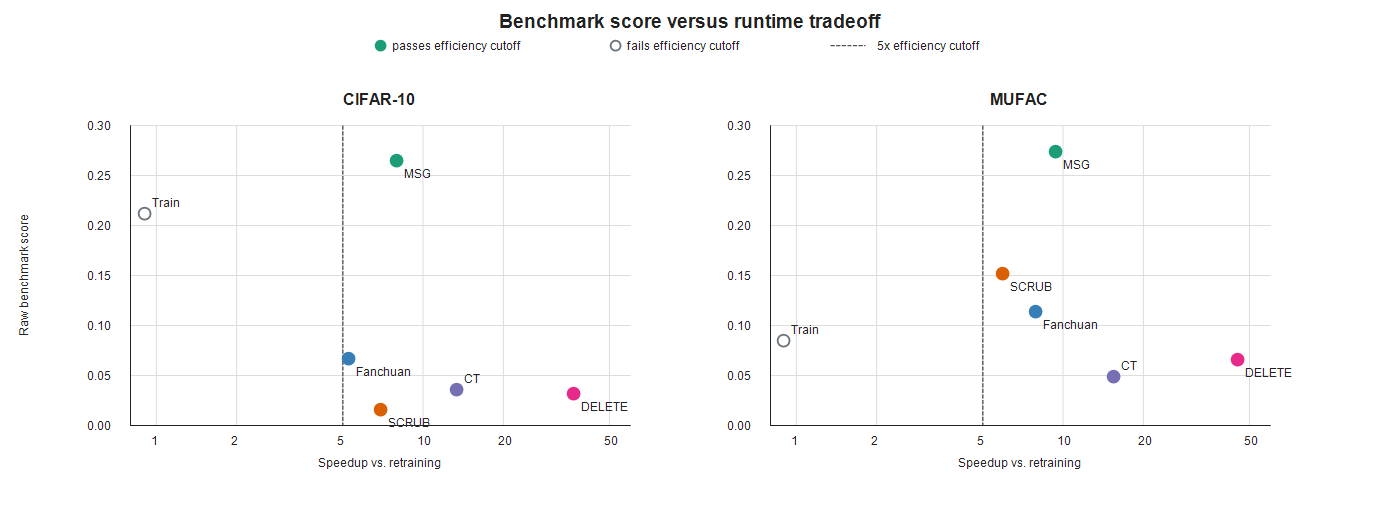
\includegraphics[width=1\linewidth]{figures/benchmark-score-speedup.png}
    \caption{Raw benchmark score versus speedup over retraining for each model family. The dashed vertical line marks the $5\times$ speedup implied by the efficiency cutoff. Filled points pass the cutoff, while the hollow training baseline remains disqualified despite a nonzero raw score.}
    \label{fig:benchmarkTradeoffs}
\end{figure}



The remaining methods each expose a different failure mode. \textbf{Fanchuan} preserves utility almost perfectly, but its forgetting quality is too weak to compete, yielding final scores of only $0.0667$ on CIFAR-10 and $0.1139$ on MUFAC despite solid speedups. \textbf{SCRUB} is much more dataset-sensitive: it performs poorly on CIFAR-10, but on MUFAC it reaches the second-best final score ($0.1522$) and the highest test accuracy ($0.5000$), while still suffering a large retain-accuracy drop to $0.6265$. This makes SCRUB interesting, but unstable. At the other extreme, \textbf{CT} and \textbf{DELETE} are the fastest methods in the benchmark, reaching roughly $13\times$ to $45\times$ speedups, yet their retain and test accuracies fall too far below retraining to remain competitive on the final score. Taken together, these comparisons suggest that fast approximate unlearning is not enough by itself; the strongest methods are the ones that preserve utility while still producing a meaningful privacy-oriented forgetting signal.

Several limitations guide our future work. First, our evaluation is constrained to two datasets, one forget-task (\texttt{forget\_mixed}), and three models per family; future research should test diverse forget-set structures (e.g., class-specific, random, long-tail) and use more seeds to better assess volatility. Second, algorithms like SCRUB require aggressive, method-specific retuning rather than a shared experimental envelope. Finally, extending benchmarks beyond ResNet-18 and incorporating Pareto or cost-aware analyses would provide a clearer view of when unlearning genuinely outperforms retraining.
\section{Conclusion}
In this report, we benchmarked several approximate machine unlearning algorithms against a retraining baseline on two image classification datasets. We also provided an overview of common unlearning approaches and the evaluation criteria used to assess them. Our evaluation focused on three key metrics: forgetting quality, utility retention, and runtime efficiency.

Our results show that while many methods achieve strong performance along one or two of these dimensions, only Masked-Small-Gradients (MSG) consistently balances all three, achieving the best overall performance across both datasets. This highlights the importance of multiple factors when considering the practical viability of unlearning algorithms, as a method that is fast but fails to forget effectively may not be useful in real-world applications, whereas a method that forgets well but is too slow will not be scalable to modern large models.

\printbibliography


%%%%%%%%%%%%%%%%%%%%%%%%%%%%%%%%%%%%%%%%%%%%%%%%%%%%%%%%%%%%
\newpage
\appendix

\section{Supplementary material} \label{app:info}
\subsection{Forget-task distributions}

The task is not class-uniform. Instead, it deterministically selects the most frequent labels in the canonical training split and removes a fixed fraction of those examples into the forget set. On CIFAR-10, where the training split is class-balanced, this produces a clean targeted deletion task: $4{,}500$ training examples are forgotten in total, with $1{,}500$ examples each from \texttt{airplane}, \texttt{automobile}, and \texttt{bird}, while the remaining seven classes are left entirely in the retrain split. On MUFAC, the base dataset is already imbalanced, so the same \texttt{forget\_mixed} construction yields a visibly skewed forgetting task: $822$ examples are forgotten in total, concentrated in classes \texttt{a}, \texttt{b}, and \texttt{c} with counts $293$, $273$, and $256$, respectively. These plots help explain why forgetting difficulty and utility preservation need not look the same across datasets: the unlearning target is balanced and structured on CIFAR-10, but inherits MUFAC's long-tailed label distribution.

\begin{figure}[htbp]
    \centering
    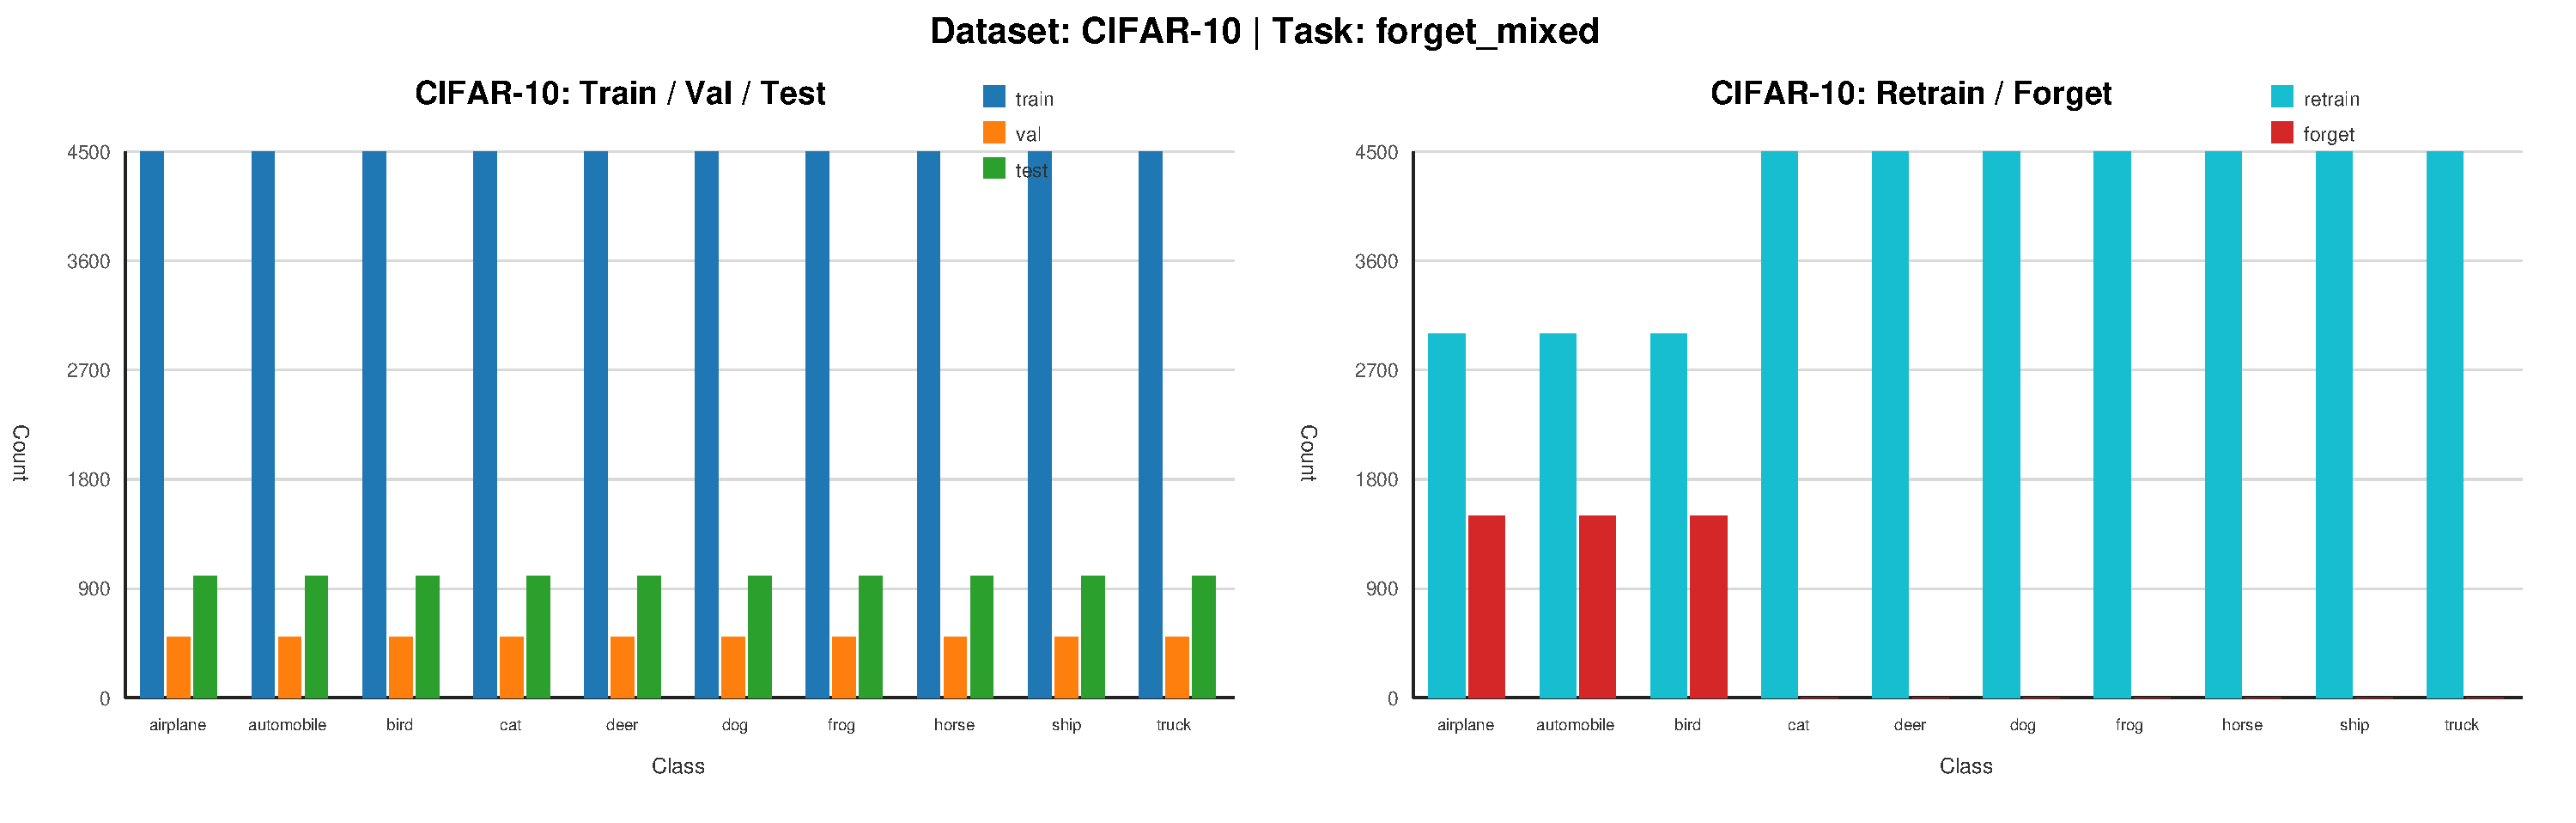
\includegraphics[width=1\linewidth]{figures/cifar10_forget_mixed_histograms.pdf}
    \caption{Class distributions for the CIFAR-10 \texttt{forget\_mixed} task. Left: the canonical train, validation, and test splits. Right: the retrain/forget partition induced by the forgetting task, which removes only \texttt{airplane}, \texttt{automobile}, and \texttt{bird} examples.}
    \label{fig:cifarForgetMixedHist}
\end{figure}

\begin{figure}[htbp]
    \centering
    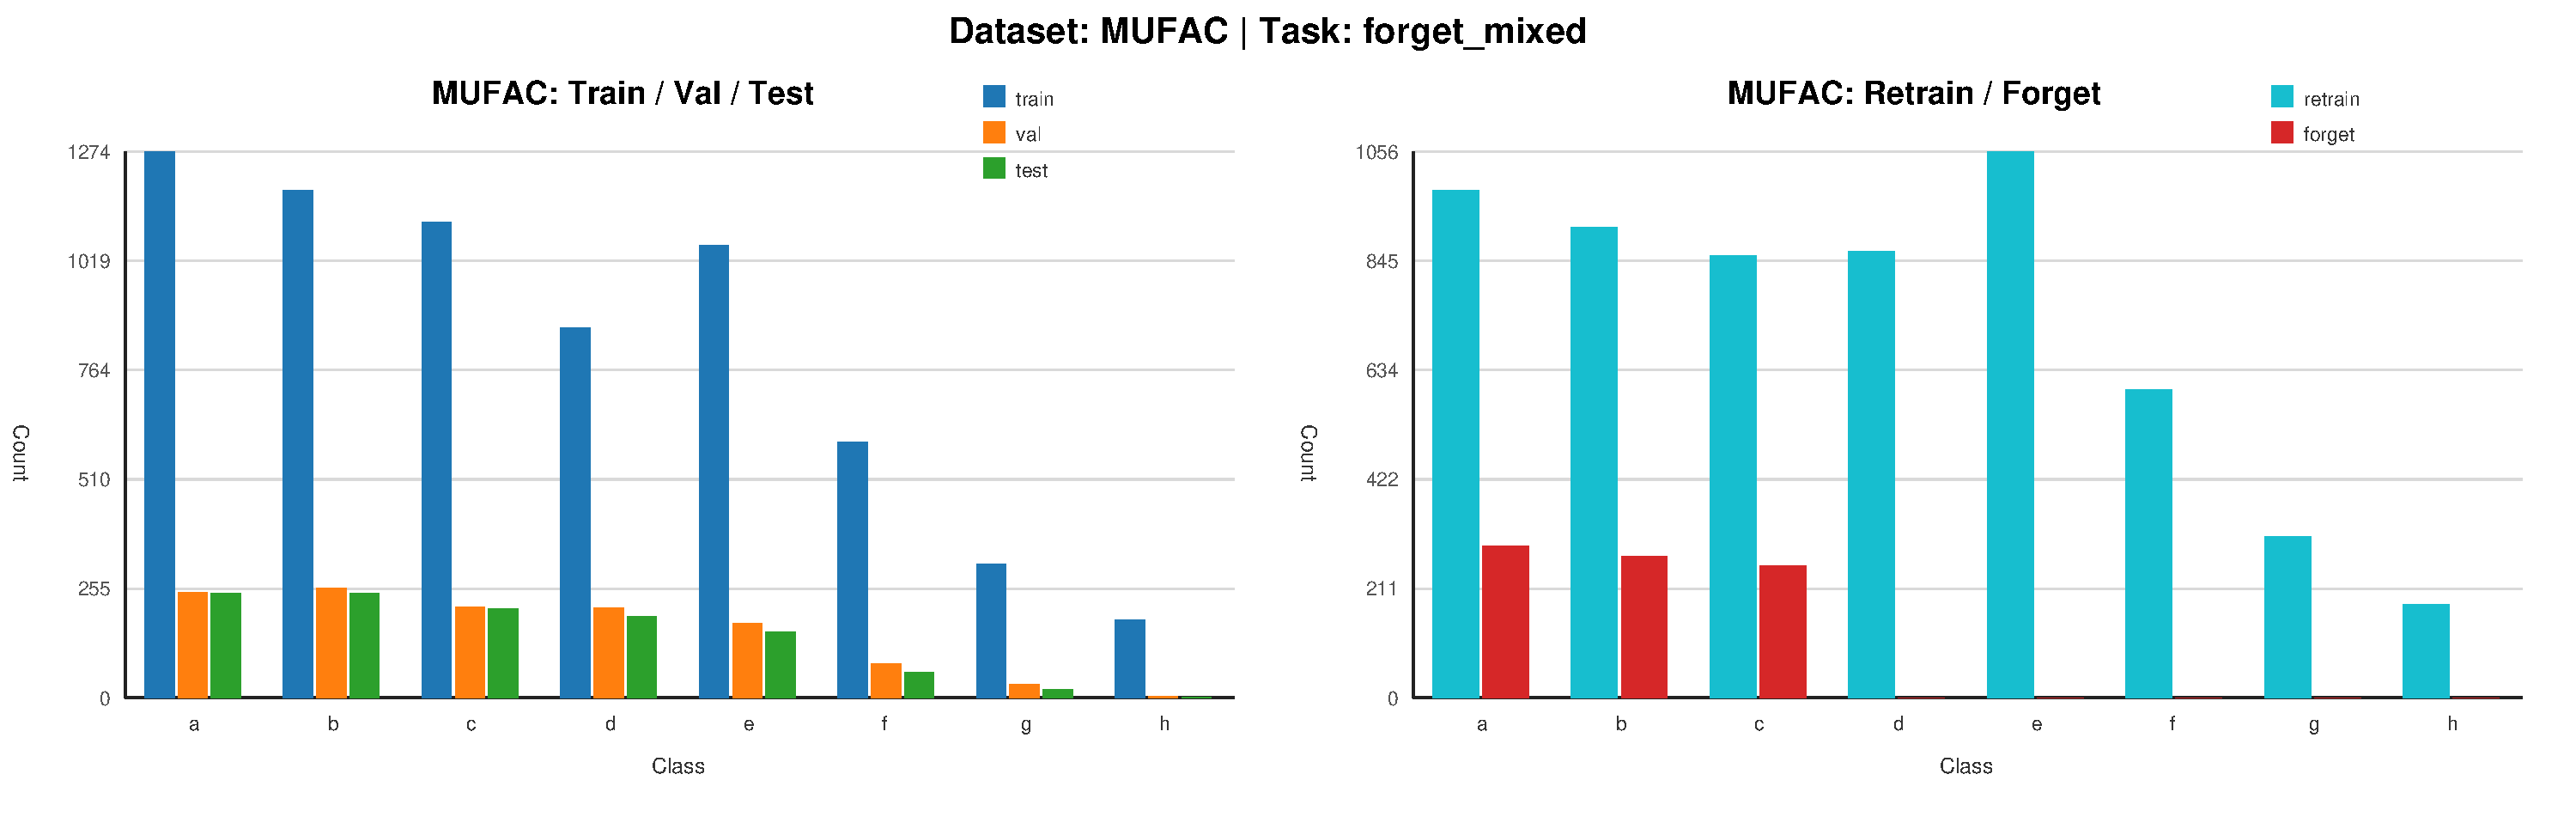
\includegraphics[width=1\linewidth]{figures/mufac_forget_mixed_histograms.pdf}
    \caption{Class distributions for the MUFAC \texttt{forget\_mixed} task. Left: the canonical train, validation, and test splits. Right: the retrain/forget partition, where the forget set is concentrated in the most frequent classes and therefore reflects MUFAC's underlying imbalance.}
    \label{fig:mufacForgetMixedHist}
\end{figure}

\subsection{Hyperparameter tuning}
\cref{fig:hyperparameterTuning} and \cref{fig:hyperparameterTuning2} show the results of our hyperparameter tuning for ResNet-18 on CIFAR-10 and MUFAC, respectively. 
\begin{figure}[htbp]
    \centering
    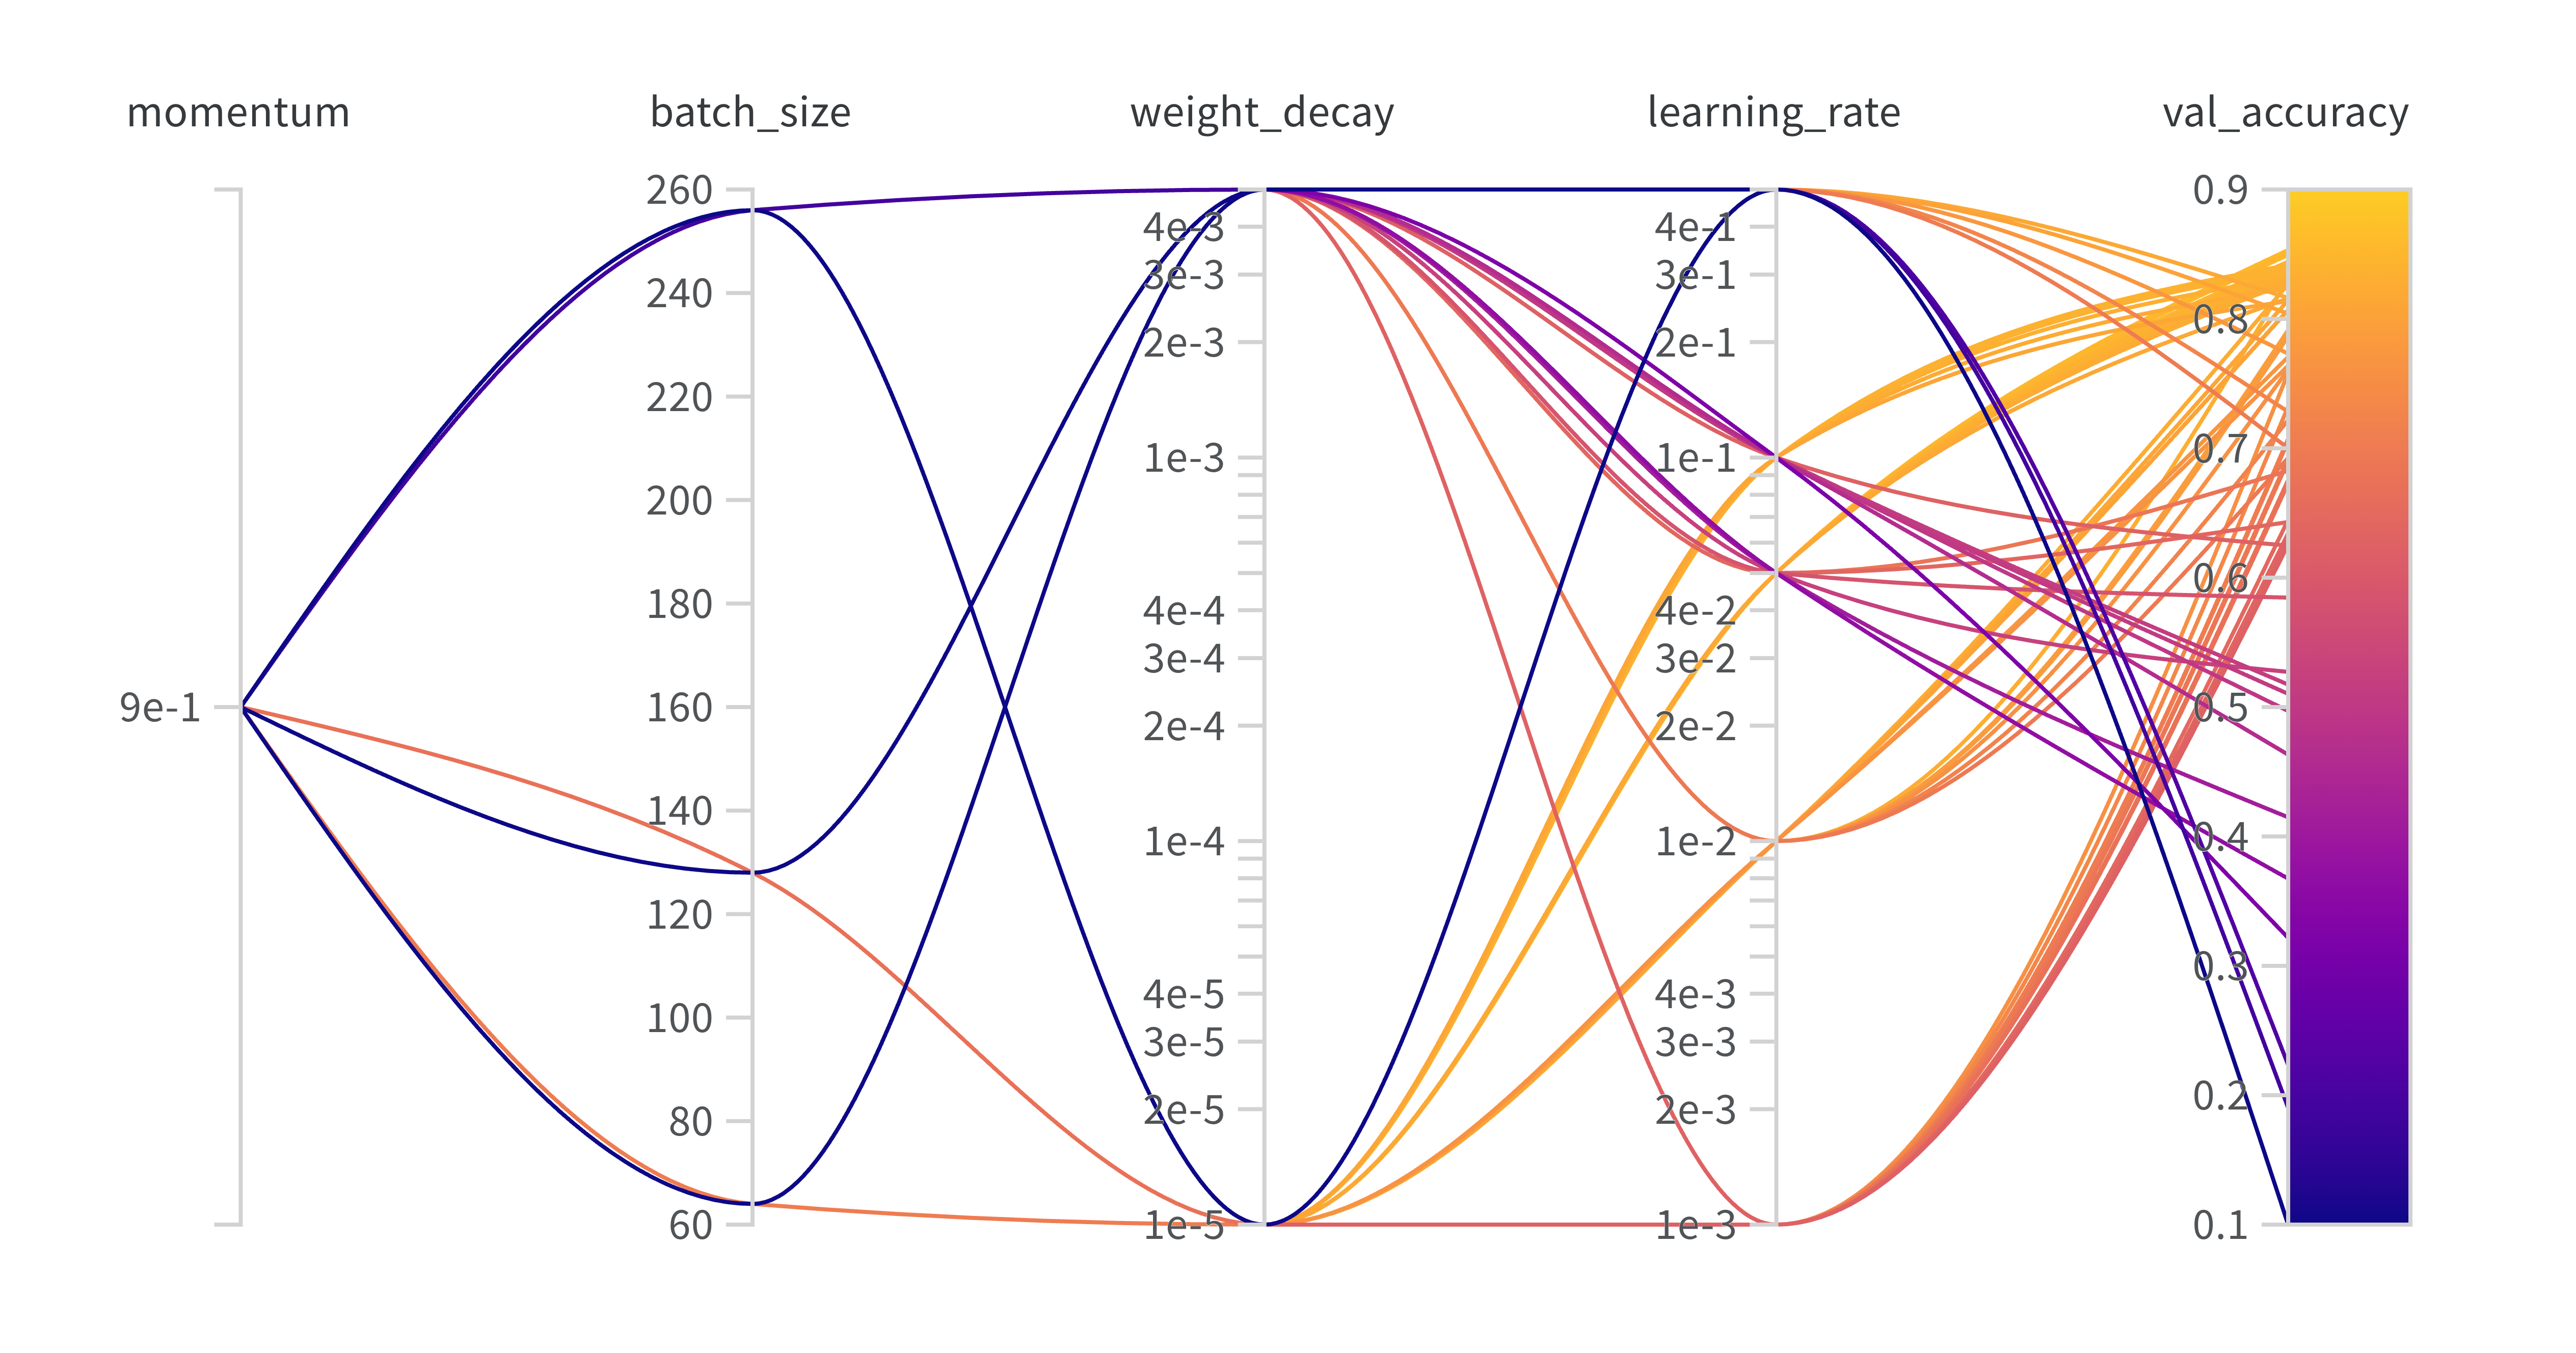
\includegraphics[width=1\linewidth]{figures/cifar-hyperparameter-tuning.png}
    \caption{CIFAR-10 Hyperparameter tuning for ResNet-18}
    \label{fig:hyperparameterTuning}
\end{figure}

\begin{figure}[htbp]
    \centering
    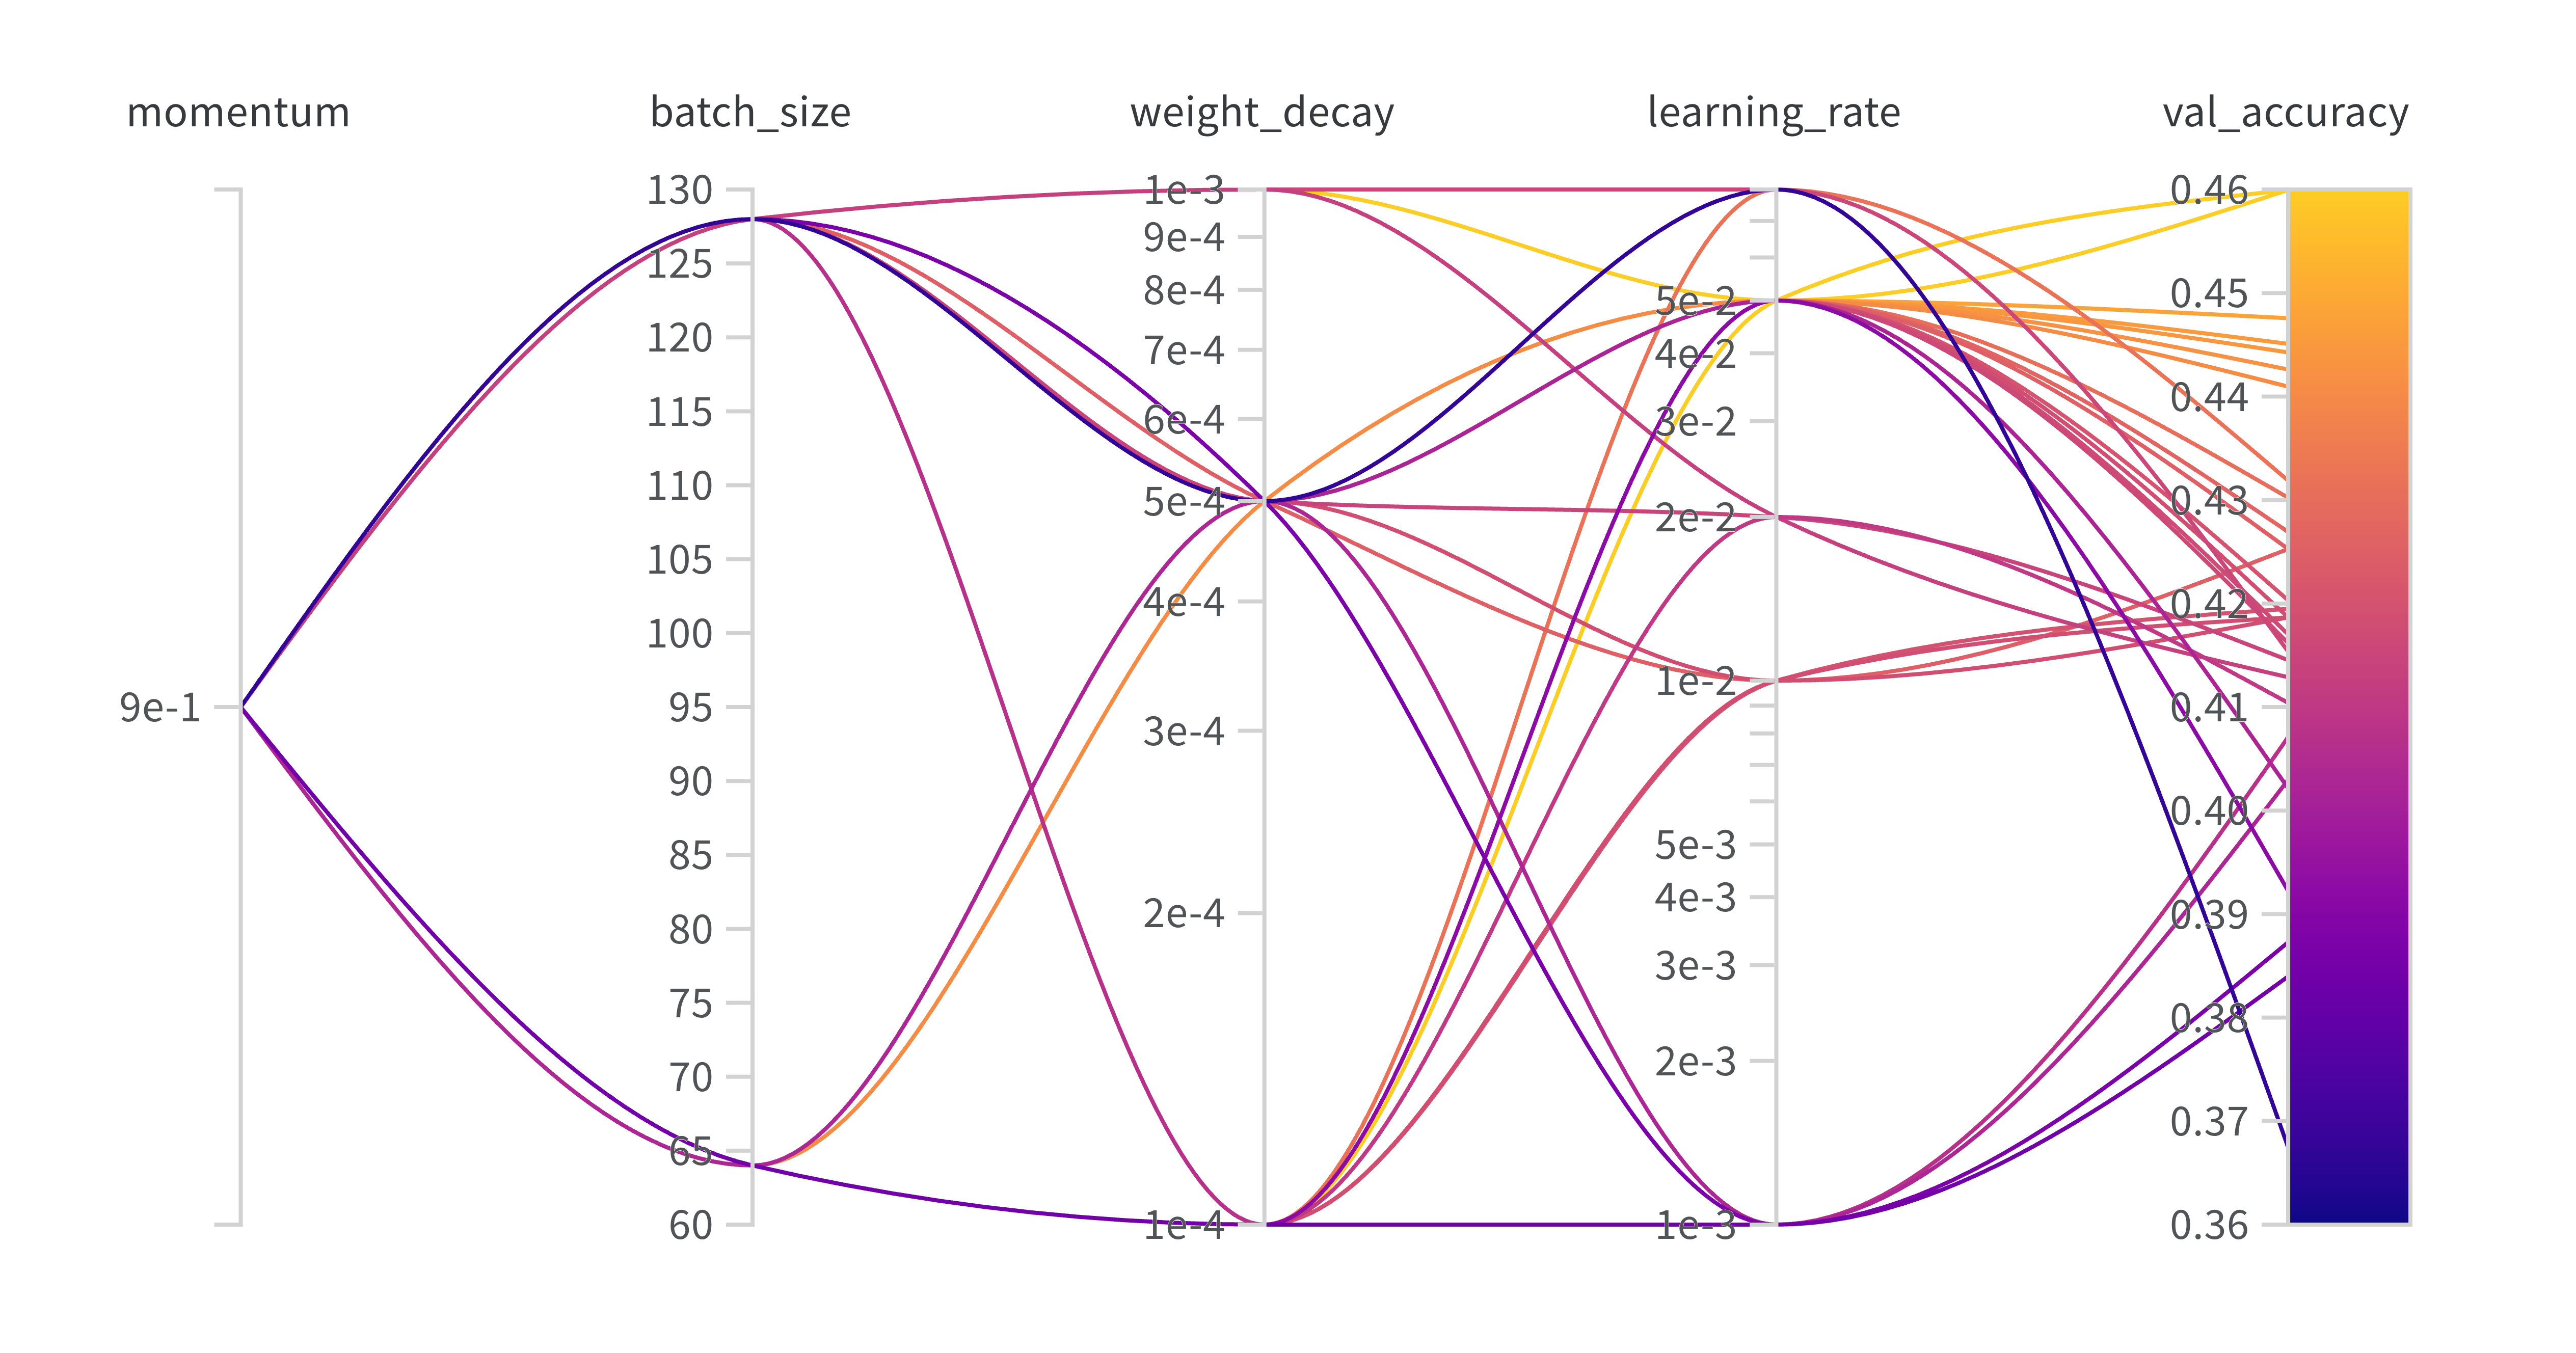
\includegraphics[width=1\linewidth]{figures/mufac-hyperparameter-tuning.png}
    \caption{MUFAC Hyperparameter tuning for ResNet-18}
    \label{fig:hyperparameterTuning2}
\end{figure}


 \end{document}
